\documentclass[12pt,letterpaper]{article}
\usepackage{float}
\usepackage{parskip}
\usepackage{hyperref}
\usepackage{graphicx}
\usepackage{setspace}
\usepackage{geometry}
\usepackage{indentfirst}
\usepackage{subcaption}
\usepackage{anyfontsize}
\usepackage[utf8]{inputenc}
\usepackage[babel]{csquotes}
\usepackage[american]{babel}
\usepackage[notes,backend=biber,isbn=false]{biblatex-chicago}

\hypersetup{
	colorlinks=true,
	linkcolor=black,
	urlcolor=black,
	citecolor=black,
}

\addbibresource{history-ia.bib}
\defbibheading{bibliography}{\section{Bibliography}}
\bibliography{history-ia}
\renewbibmacro*{cite:ibid}{\printtext[bibhyperref]{\bibstring[\mkibid]{ibidem}}}
\geometry{letterpaper, portrait, margin=1in}
\doublespace
\graphicspath{{../imgs/}}

\title{Involvement of the 1980 Moscow Olympic Games Boycott in the Cold War}
\author{Tynan Purdy}
\date{May 2019}

\begin{document}

\parindent=0.5in

{\fontsize{12}{14.4}
	{\singlespace
	    \pagenumbering{gobble}
	    \maketitle
	    \begin{center}
	    002129-0002 \\
	    \vspace{4mm}
	    IB History HL IA \\
	    \vspace{4mm}
	    Words: 2130 \\ % words
	\end{center}
	}
}	

\newpage
\tableofcontents
\pagenumbering{arabic}
\newpage

\section{Evaluation of Sources}
% ~500 words
% introduction - 2 sources, research question, explanation of sources (couple sentences for all of this)
% specifics of the sources

How did Russian involvement in the Afghanistan conflict lead to the US boycott of the 1980 Olympic Games? With all the tensions over events in Afghanistan, the ongoing Cold War, as well as boycotts lead by the Carter Administration on the '80 Games,\footcite[559]{guttmann_cold_1988} even the most sacred and peaceful international gathering was affected. This investigation aims to establish and explain the relationship between the Afghan conflict, the USA and USSR, and the unique circumstances of the Moscow Summer Games in 1980 in relation to the Cold War.

\subsection{Source 1: \citetitle{guttmann_cold_1988}}
% discuss V and L thru C and O and P
% OPcVL

\citetitle{guttmann_cold_1988} offers a political context for the events significant to the investigation. It summarizes the political events surrounding the Olympic Games and actions of nations involved in the Cold War that pertained to the Games. With knowledge of not just the immediate political context of the Games, such as the boycotts and Russian invasion of Afghanistan, but also the previous abstinence of Russia from the Games and the process of them joining the International Olympic Committee\footcite[555-558]{guttmann_cold_1988}, the biases, mindset and preconceptions of the American and Soviet citizens can be better approximated. Author of the article, \citeauthor{guttmann_cold_1988}, is an esteemed professor at Amherst College, with five degrees and a focus on literature and American studies. He teaches ``Sport and Society'' as well as ``The Nazi Olympics'' based on his research and experience in those topics, alongside his American literature courses. The purpose of \citeauthor{guttmann_cold_1988}'s article is to provide a comprehensive narrative of the interactions of Cold War politics and the Olympic Games. \citetitle{guttmann_cold_1988} provides a political narrative overview for the investigation and points to several key events that may have connected the Games and the Cold War events.

\subsection{Source 2: \citetitle{eskenazi_u.s._1980}}
% ditto
% OPcVL

\citetitle{eskenazi_u.s._1980} is an article from The New York Times by reporter \citeauthor{eskenazi_u.s._1980}. This is a first hand account of the gold medal hockey game between the USA and USSR men's hockey teams. It has the advantage of being a primary document, giving an authentic impression and emotional snapshot of the game from an American spectator viewpoint. The author has the real context of the American people at the time, allowing him to give remarks such as ``Few victories in American Olympic play have provoked reaction comparable to tonight's decision at the red-seated, smallish Olympic Field House''.\footcite{eskenazi_u.s._1980} This article provides insight into what got the American's attention in the game, specifically certain alleged uncalled fouls by the Russians as well as a brag that the US team got their winning tactics from the Russian's themselves. The comments in the article reveal the novelties of the US USSR rivalry, contributing to the investigation well. The article is limited by it's format as a written article, which cannot convey nearly as much emotional information as video. However that shortcoming will be made up for as original footage of the game will also be considered in the investigation. The Miracle on Ice is an example of the the United States using the Olympics to publicly shame the USSR, a key component of the investigation. 

Words: 507

\newpage
\section{Investigation}

The 1980 and 1984 Olympic Games were some of the most complicated and dramatic in history due to a relentless series of boycotts having to do with events in the ongoing Cold War. It was particularly strange that the Olympics be at all involved in the Cold War as the International Olympic Committee had aimed to be an entirely apolitical organization,\footcite[3]{keys_political_2017} and even lead several campaigns to convince countries to promise not to boycott the Olympics. In 1979, just leading up to the 1980 Games, the USSR began its military intervention in Afghanistan, which the Afghan government requested in order to pacify its growing rebellious groups.\footcite[559]{guttmann_cold_1988} The intervention was a move the United States had been attempting to prevent, in one strategy, by boycotting the 1980 Moscow Olympic Games. In return the Soviet Union boycotted the 1984 Los Angeles Games. With limited forceful or military actions left to use against the USSR, President Carter turned to an Olympic boycott as a public shaming to pressure Russia out of Afghanistan. 

\subsection{Soviet Union}
The Soviet Union had good reason to want to intervene in Afghanistan, as the potential addition of Afghanistan into the Union would add considerable wealth and a strong proportion of power in the Asian continent, a merger that China and Pakistan were afraid of.\footcite[24-25]{urban_war_1990} In the late 70's specifically, the government of Afghanistan in Kabul struggled with growing rural rebel groups and the People's Democratic Party of Afghanistan (PDPA) after the assassination of Mir Akhber Khyber in the April Revolution of 1978.\footcite[15]{urban_war_1990} The April Revolution kick started a period of active revolt and instability in Afghanistan, eventually prompting Soviet intervention. The Brezhnev Doctrine, a foreign policy of the USSR at the time, stated that for ``an ally state about to fall to anarchy or outright hostile forces, intervention was an essentially defensive, reactive move to forestall such a humiliating and potentially dangerous outcome'' \citeauthor{galeotti_afghanistan:_2012}.\footcite[11]{galeotti_afghanistan:_2012} This part of the Doctrine gave the loophole for Russia to claim the right to intervene in Afghanistan. On December 28, 1979, Kabul sent its request to Russia for a military intervention in Afghanistan.\footcite[559]{guttmann_cold_1988} The Soviet Union readily supported the PDPA as the communist party of Afghanistan, just as they had supported the Chinese Communist Party in the later stages of the Chinese Civil War. The Soviet support helped the PDPA to rise above other guerrilla opposition groups in Afghanistan such as the Hezb-e-Islami and the Afghan People's Liberation Organization, supplying a large portion of Afghanistan's military equipment and technical training as listed in Figure \ref{fig:requests}\footcite[8]{galeotti_afghanistan:_2012}. Among those who were against the Soviet Union's intervention, The United States were the most vocal and active in their disapproval.

\begin{figure}[H]
	\centering
	\caption{Afghan military aid from Russia}
	\label{fig:requests}
	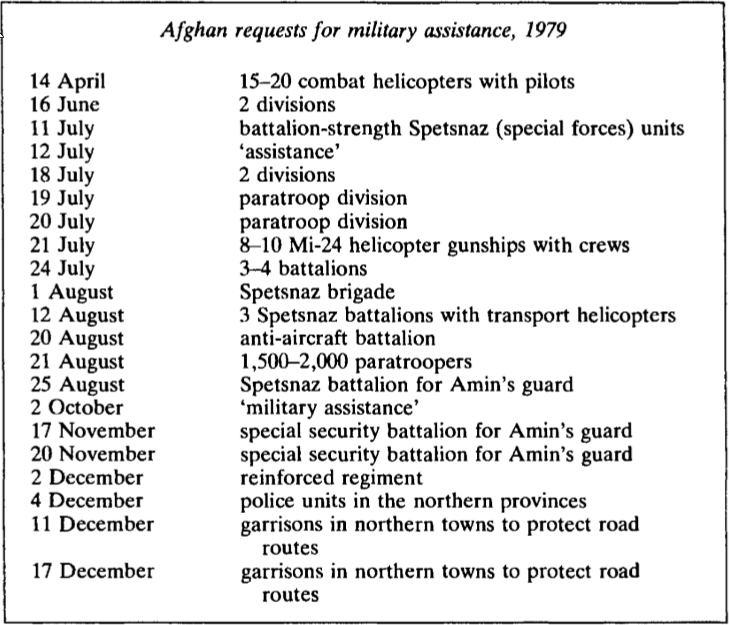
\includegraphics[width=.6\linewidth]{requests}
\end{figure}

\subsection{United States}
The United States' continued `war on communism' was falling short in the Afghan region. The Peace Corps had been deployed to Afghanistan with aid, but were called back after the US ambassador Adolph Dubs was kidnapped by the Settem-e-Melli terrorist group and, soon after, was killed in crossfire as his hotel was attacked.\footcite[29]{urban_war_1990} With no more military presence in Kabul, the United States transitioned to social, political, and economic motivations to get Russia to end their intervention. \citeauthor{kanin_olympic_1980} details, ``It is important to keep in mind that the Olympic boycott was only one of the economic and political sanctions making up the US response to Afghanistan. The others, which included grain embargoes, restrictions on sales of high technology goods and processes, and curtailment of the whole gamut of scientific and cultural exchanges, involved issues more important to the Soviet economy, but did not provide the potential for public embarrassment the way the Olympics did.''\footcite[6]{kanin_olympic_1980} The US could erode Russia economically, but to achieve a public retribution, it needed a large scale shaming, which the Moscow Olympics gave the perfect opportunity for. President Carter stated in a letter to Robert J. Kane, the president of the US Olympic Committee at the time, that the US must ``make clear to the Soviet Union that it cannot trample upon an independent nation and at the same time do business as usual with the rest of the world.''\footcite{smith_president_1980} On January 20, 1980, President Carter requested that the IOC move the games from Moscow unless Russian troops were extracted from Afghanistan within a month, but the point of return on contracts had already passed, leaving only a boycott for protest.\footcite[7]{kanin_olympic_1980}\textsuperscript{,}\footcite{smith_president_1980} Part of the public shaming of the Soviet Union, while not technically planned, was the `Miracle on Ice', the men's ice hockey gold medal final between the US and USSR. \citeauthor{eskenazi_u.s._1980} of the New York Times wrote the headline \citetitle{eskenazi_u.s._1980}. The game featured no shortage of national rivalry and disposition against the Soviets. The US even complained about an uncalled foul, even though they won the game. ``The Russians had one when Sergei Makarov punched the puck past Craig while fans screamed in vain for Referee Karl-Gustav Kaisla of Finland to notice an American who was being held.'' \citeauthor{eskenazi_u.s._1980}. 

\subsection{International Olympic Committee}
	None of these boycotts or global political motivations were at all pleasing to the International Olympic Committee. While Olympic boycotts had occurred in the past, specifically on the 1976 Montreal Olympics,\footcite[559]{guttmann_cold_1988} the IOC rules had stated for years that national Olympic Committees must be politically independent from their government, a rule Russia struggled with as it joined the Olympics in 1951.\footcite[557]{guttmann_cold_1988} The Moscow Games were some of least successful in the IOC ideology of global community and setting aside issues when ``More than 60 countries stayed home in 1980, inflicting a grievous blow to the IOC’s global and universalist pretensions,'' \citeauthor{keys_political_2017}.\footcite[1]{keys_political_2017} The IOC president at the time, Juan Antonio Samaranch, lead multiple campaigns to the United Nations in 1981 and 1985, when similar boycotts on the Los Angeles Games were lead by Russia. The campaigns requested a declaration to protect the Olympic Games from boycotts, but the IOC's strategy was flawed from the beginning. Not only was the IOC plea to the political leaders of the world hypocritical because of its political nature, but the UN was in no position to be of aid during their limited effectiveness in the midst of the Cold War.\footcite[2]{keys_political_2017}
	
\subsection{Conclusion}
The Moscow Olympic Games of 1980 demonstrated how, despite attempts, the Olympics do have political context, and are not isolated in a Utopian bubble of peace. The Soviet Union intervention in Afghanistan was a strategic and calculated move, but publicly received an assault of criticism, especially from the United States. President Carter responded with economic sanctions on  and political retaliations, leading a boycott with over 60 nations of the 1980 Moscow Olympic Games, which embarrassed the USSR and the IOC. An event as prestigious and culturally important to the whole world as the Olympic Games will inevitably have impacts and be impacted by the rest of the world. Whether the Moscow Games boycott achieved its purpose or had any important or measurable impact on Russia is another question, but it can be said that, despite the dream of an apolitical and friendly global competition, the Olympic Games did have actively political consequences in the case of the 1980 Moscow Olympic Games. 

Words: 1215

\newpage
\section{Reflection}
There were a few specific tools I found that, when put together, formed the ultimate historian research paper arsenal that allowed me to have all accessible and digital sources. Finding adequate and genuine source material can be immensely difficult and time consuming for historians. Emory University was kind enough to allow me to find books and articles at their Woodruff Library, but I could not access copies of sources off-campus. I found publicly accessible PDF copies of any source I wanted on Sci-Hub, which is an open source repository with institutional access to many of the journals and repositories of academic papers that often restrict access behind a pay wall. To collect my sources, I used Zotero, a fantastic software that collects bibliography information automatically, using any of the standard identification systems such as DOI or ISBN. The final component that made everything to do with citations and citing correctly according to the Chicago standards was \LaTeX{}, a text markup environment that compiles PDF documents, and has hundreds of available packages to add functionality. I added a set of packages that allow me to automatically cite and create a bibliography in Chicago format, using a bibliography file I exported directly from Zotero. These tools together made the research and writing process far smoother that it would have been otherwise. Although technology has been a great aid to me during this process, it did hurt in other areas. When attempting to access a primary document from an online archive, the original video of President Carter calling for the boycott, I could not watch it because the video was encoded with Adobe Flash, which simply refused to run on my computer. Technology is great, but it moves so fast that older formats are left behind, rendering content lost in the process. As is common, my research topic went through many iterations before its final form. I started at explaining the general cultural rivalry between the US and Russia, eventually focusing specifically on film and sport, then just sport, the Olympics, and finally the 1980 games in particular. While I cannot be sure of much in history, I am sure my biases surround this investigation. Just as I assess the sources used in the investigation, the reader must asses me when reading what I try to present as neutral, but is my opinion produced from my biases. 

Words: 394

\newpage
\nocite{*}
\printbibliography

\newpage
\section{Appendix}
\listoffigures

\end{document}